% !TEX root = tesis.tex

\chapter{Detección de partículas energéticas\\ solares en el \emph{SciCRT}}
\chaptermark{Detección de partículas}
\label{chap:cuatro}
\section{Desempeño del \emph{SciCRT} como detector de RC}



\begin{figure}
        \centering
        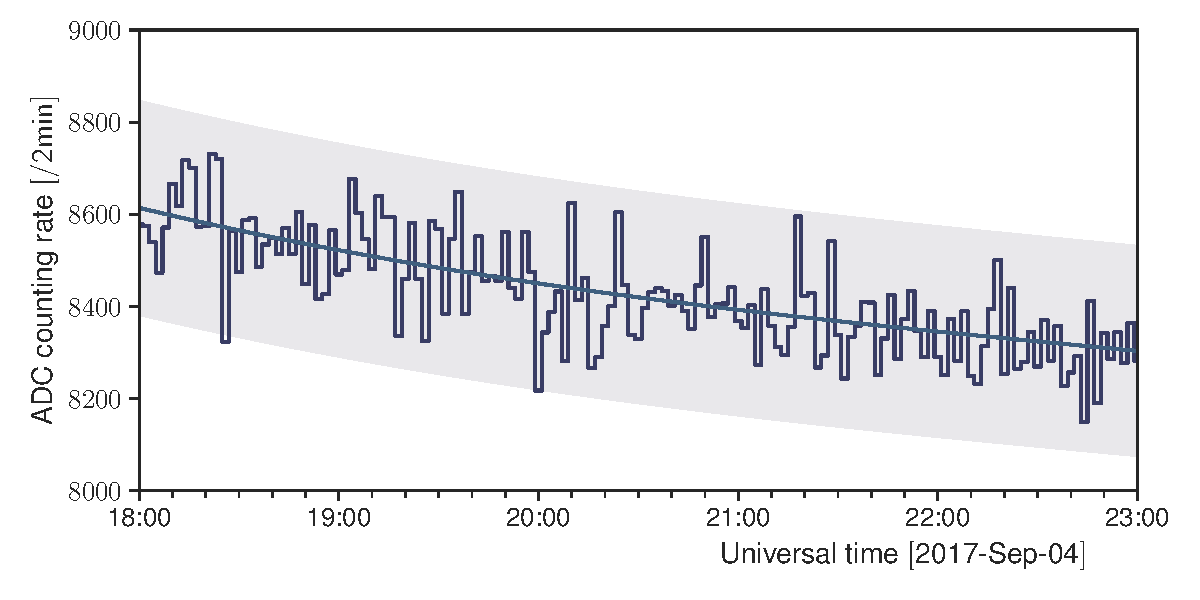
\includegraphics[width=\textwidth]{neutron-170904.pdf}
        \caption{Perfil temporal de eventos registrados por el \emph{SciCRT} el \num{4} de Septiembre de \num{2017}. El área sombreada representa el nivel de $3.0\sigma$.}
        \label{fig:september-04}
\end{figure}

\begin{figure}
        \centering
        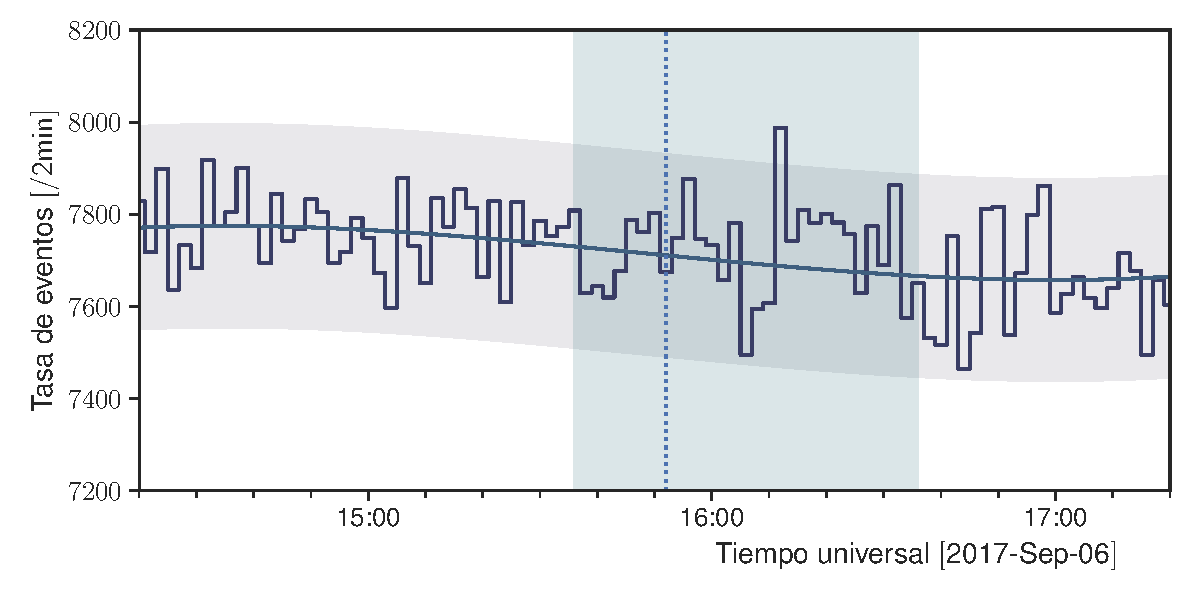
\includegraphics[width=\textwidth]{neutron-170906.pdf}
        \caption{Perfil temporal de eventos registrados por el \emph{SciCRT} el \num{4} de Septiembre de \num{2017}. El área sombreada representa el nivel de $3.0\sigma$..}
        \label{fig:september-06}
\end{figure}
